\chapter{Character Management}

\section{Character Types and Character Templates}
Anathema distiguishes between character types and character templates. "`Character type"' denotes the general disposition of your character, her "`race"' if you will - whether she is a Lunar Exalt, a Solar, or a common mortal. The character template, on the other hand, describes the rules used for character creation and advancement (point costs, points granted and so on) and gives a general idea of her background.

Templates are tied to the character types. For many types, there is only a single template available, but some -- like the ever-prolific Dragon-Blooded -- come with many different variants.

Since they deal with rules used for your character, the availability of a certain template also depends on the rules you want to use.

\section{Character Creation}
From the "`New"' dialog select "`Character"' to reach the template selection screen, shown in \ref{fig:TemplateSelection}

\begin{figure}
	\centering
		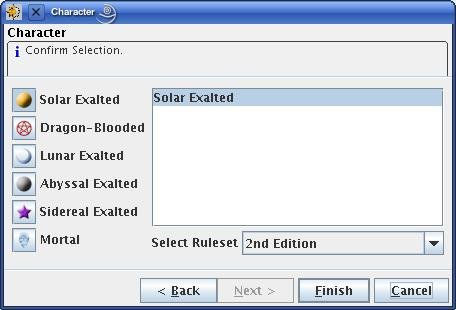
\includegraphics[width=1.00\textwidth]{images/TemplateSelection.png}
	\caption{Selecting rules, type and template for a new character}
	\label{fig:TemplateSelection}
\end{figure}

There, select the character type you want to create and the ruleset used. The field on the right hand side will now show a list of character templates available for your selection. Choose one, and confirm your selection by clicking the "`Finish"' button below. Don't worry about further details for now, everything else is controlled in the window that is now opening.

\section{Common Controls}
Some controls are shared by different screens. They are collectively explained here.

\subsection{Adjusting trait values}
Throughout Character Managent, you will notice rows of dots as seen in figure \ref{fig:TraitControl}. They are used to adjust your character's trait values and are hence called 'trait controls'

To select the number of dots assigned to a certain trait, just click on the dots and they will be filled in. Clicking the last dot to be filled will fill all previous dots as well. (Obviously. Clicking on the fourth dot will fill 4 dots, not just the one you clicked.) Alternatively you can press the mouse button and drag the appearing rectangle until the trait is set to the amount you want it to be. 

If you want to lower a trait value, click on new value, or, again, use the press-drag selection. To set the value to 0, click close to the beginning of the first dot. 

Most trait controls will not allow to select illegal values, so if a click yields no reponse or the dots covered by the rectangle are not selected, the values are most probably not allowed by the rules. (Try, for instance, lowering a favored Ability to zero dots.)

\subsection{Caste and Favored Traits}
On the attributes and abilities tabs, you will note a button in front of each trait control. (Refer to figure \ref{fig:TraitControl} once again for a visual impression.)

The state of this button indicates the state of the trait: Standard, Caste or Favored. An unmarked button denotes the default case, a standard trait. Caste traits are indicated by your characters Caste mark, while favored traits are indicated by a "`dot"' just like the ones used in the trait controls.

To toggle between standard and favored states, click the button. Anathema will then take care of minimum values. Caste traits can't be toggled off, but are set automatically by selecting the appropriate caste instead.

\begin{figure}
	\centering
		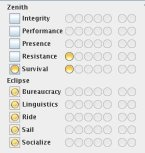
\includegraphics{images/TraitControl.jpg}
	\caption{Trait Controls with favorization (upper block, 5th row) and Caste abilities (lower block).}
	\label{fig:TraitControl}
\end{figure}

\subsection{Removeable Entries}

\begin{figure}
	\centering
		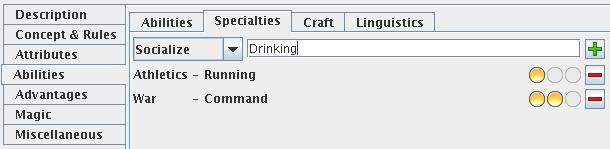
\includegraphics[width=1.00\textwidth]{images/RemovableEntries.jpg}
	\caption{Specialties, an example of removable entries}
	\label{fig:RemovableEntries}
\end{figure}

Several parts of the character allow for custom values to be defined.

Many of these screens use the "`removable entry"' control scheme, shown in figure \ref{fig:RemovableEntries}.
The top row allows for an entry to be specified and added by clicking the add-button. The entry will then be shown in the area below. To remove it, click the remove-button next to the entry.

Most screens using this control will add some spice - Backgrounds, for example, allow for the value of the background to be changed, whereas a Lunar's animal form will ask you to not only specify a name, but also to give values for the form's strength and stamina.

\subsection{Overview}
The Overview on the bottom left will keep track of choices made and points spent, automatically adjusting if you change things. 

The overview knows two separate states, one for character creation and another for experienced characters. They will be covered in their relevant sections.

\section{Navigating the character}
Cascaded tabs are used for navigating the different aspects of your character. The left of the screen shows the general areas, each of which may contain sub-areas. Magic, for example is split in Charms, Combos and Sorcery, while Attributes are just that.

We'll cover the different areas in the next few sections, for now, all you need to know is that you can navigate through both sets of tabs by left-clicking them.

\section{Character Creation}

\subsection{Overview during Character Creation}
While your character is being created, the overview shows the free dots and bonus points spent.

There are entries for the common elements shared by every character type and an additional tracker for miscellaneous spendings and those unique to the template chosen.

Colors and font show the state of the item displayed: Purple indicates that you still have free dots remaining, 
while black means that everything allotted is spent. Items on which you spent bonus points are shown bold. 

All point spendings are calculated automatically using a best-build calculator, so you need to worry neither about the attribute group priorization nor about bonus point choices.

The total bonus points spent are shown in the overview's last line and updated for every choice you make. If the total becomes red, you have overextended the allowed amount.

Number in parentheses indicate that the characters absolute maximum has somehow been raised above the maximum.(eg. additional bonus points granted through flaws), while a second number delimited by a "+" notifies you of additional points to spend. Common examples are backgrounds like "`Sorcery"' and "`Necromancy"', which allow for additional spells to be learned.

\subsection{Abilities}
\subsubsection{Craft}
While listed in its appropriate group on the main "`Abilities"' screen, handling of the craft ability actually differs from other traits.

Crafts are handled on a separate tabinside the Abilities window (shown in figure \ref{fig:crafts}), where you can specify which crafts your character knows, choosing from a range of pre-specified entries or adding your own. As such, the Craft skill in the main tab is locked from change. Its shown value is the maximum of all the subskills' values.

The only setting allowed there is changing favored state of the ability. Setting the ability to "`favored"' might change the values of the crafts on the specialized tab: If your overall Craft trait is at 0 dots, the first craft specified will have it's value set to 1.


\begin{figure}
	\centering
		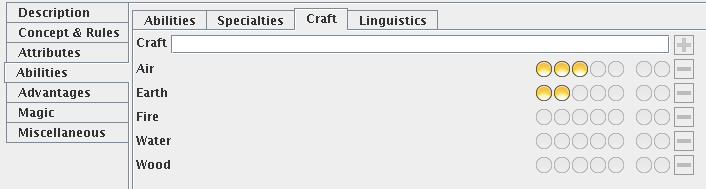
\includegraphics[width=1.00\textwidth]{images/crafts.jpg}
	\caption{Crafts Screen}
	\label{fig:crafts}
\end{figure}

\subsubsection{Specialties}
Specialties also have a screen of their own. Use the drop down list to find the Ability, then type the Specialty name into the box and press the green + button, just with regular removeable entries.

You can then select the number of times the specialty was learned by setting the dots. If you try to add an identical specialty later on, Anathema will automatically add one dot to the existing one, if possible, or ignore the addition, if not.

\subsubsection{Linguistics}
The last screen in the abilities section, Linguistics, allows you to choose the languages spoken by your character.

You can choose from the pre-defined language families or enter barbarian languages by typing in the box. Since Anathema doesn't handle native languages, the number of language-slots available is 1+(Linguistics).

\subsection{Magic}
The Magic section allows you to choose Charms and Spells, and create Combos, each on a separate page. Some views, like Necromancy and the Lunars-only "`Beastform"' screen may not be available, depending on your character and ruleset.


\subsubsection{Charms}The Charms screen is largely identical to the separate Cascade function described earlier. Obviously, there is no option to select the ruleset (it's pre-set to the one you chose at character creation) and not all charm types are available. Most characters are limited to their own type and Martial Arts, only Eclipse caste solars and Abyssal Moonshadows will see all the types. 

In addition to the functions demonstrated by the Cascades, the Charms view is used to learn charms for your character. To support this, charms in this screen have two related but separate states: Learned/Unlearned and Learnable/Not Learnable. 

Learned/Unlearned is distinguished by the charms body color, anything but white indicating learned charms. Learning and unlearning both is done via a single click on the charm. The effect triggered is indicated by the mouse cursor.

Whether a charm is learnable at all is shown by its transparency: If the charm appears to be greyed out, your character cannot legally learn it because he has not yet met all prerequisites. Clicking it will have no effect if your character doesn't already know it, but if it is already learned, you can still unlearn it.

Some charm trees show translucent entries which can not be learned. The more common variant shows text like "`2 Athletics Excellency Charms"'. These are placeholders for several other charms that could be selected to fulfill the precondition and cannot be learned on their own. Less often seen are trees with preconditions from other groups. These are displayed as fully translucent boxes with the external charm's name in it.

Anathema will automatically check whether these conditions are satisfied and set the learnable state of the dependent charms accordingly. 

\begin{figure}
	\centering
		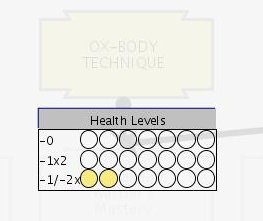
\includegraphics{images/OxBodyTechnique.jpg}
	\caption{Controls for Ox-Body Technique}
	\label{fig:OxBodyTechnique}
\end{figure}

Some Charms differ from the standard controls in that they cannot be learned by a single click. These charms have details-boxes, which allow to control certain parameters of the charm. Ox-Body Technique is an excellent example of this. 

Depending on the nature of the cascade, the details box needs to be expanded with by clicking a button below the charm itself. The Charm tree will then gray out and present to you the details.

With Ox-Body technique and similar "`multi-learnable"' Charms, they are not unlike a set of trait controls and allow you to chose the number of times you wish to purchase the effects of the charm. You can return to the standard view at any time by clicking anywhere outside the details-display.

Other flavours include "`multi-effect"' and "`sub-effect"' Charms. Multi-effect Charms are those that come in several variants with only very limited change, with each variant being a Charm of its own. The most classic example is "`[Type] Exalt Ways"' from the sidereal-level "`Prismatic Arrangement of Creation"' martial arts style, of which 22 different variants exist.

Sub-effect charms, on the other hand, are single charms with several additional Effects available, some of which might come free with the Charm's purchase.

When details of either of these types are displayed, no trait controls are shown. Instead, the program displays a list of available effects. Effects are selected and deselected by a single click, with those already chosen marked in your character's color.

\subsubsection{Spells}
\begin{figure}
	\centering
		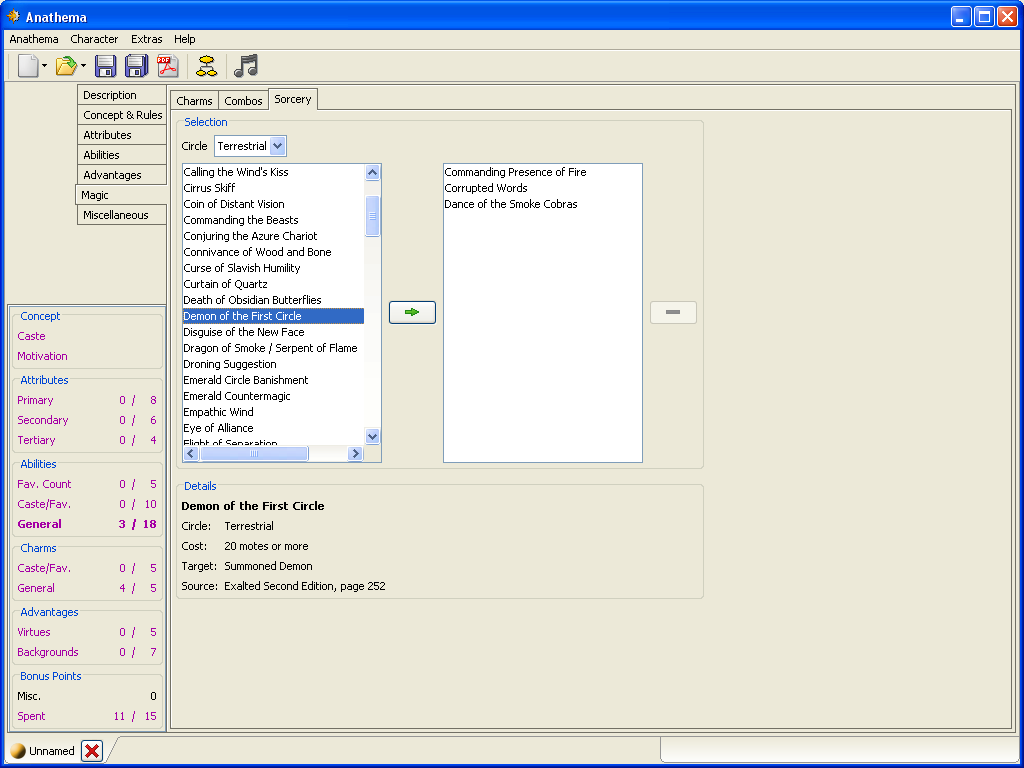
\includegraphics[width=1.00\textwidth]{images/Spells.png}
	\caption{Sorcery Screen}
	\label{fig:Spells}
\end{figure}

The Spell screen shows two lists of spells. The left-hand list contains the available spells, with those not eligible for your character grayed-out, while the right-hand list contains the spells already learned.

Spells can be learned by selecting them in the left list and clicking the green arrow. To unlearn a spell, select it, then click the red "-". 

The filtering options above the lists only applies to the left-hand one.


\subsubsection{Combos}
Combo creation is similar to spell selection: Simply select one charm at a time from the box on the left, and click the green arrows to add it to the current combo, displayed on the right. 

After all Charms have been selected, enter a name and short description of the Combo, then click the green check mark to finalize it. The bottom button can be used to clear the combo currently edited and start over. 

There is some intelligence to the selection box that grays out ineligible Charms once you begin your composition. This system only covers the bare rules, not the intricate details of inter-charm comboing.

\begin{figure}
	\centering
		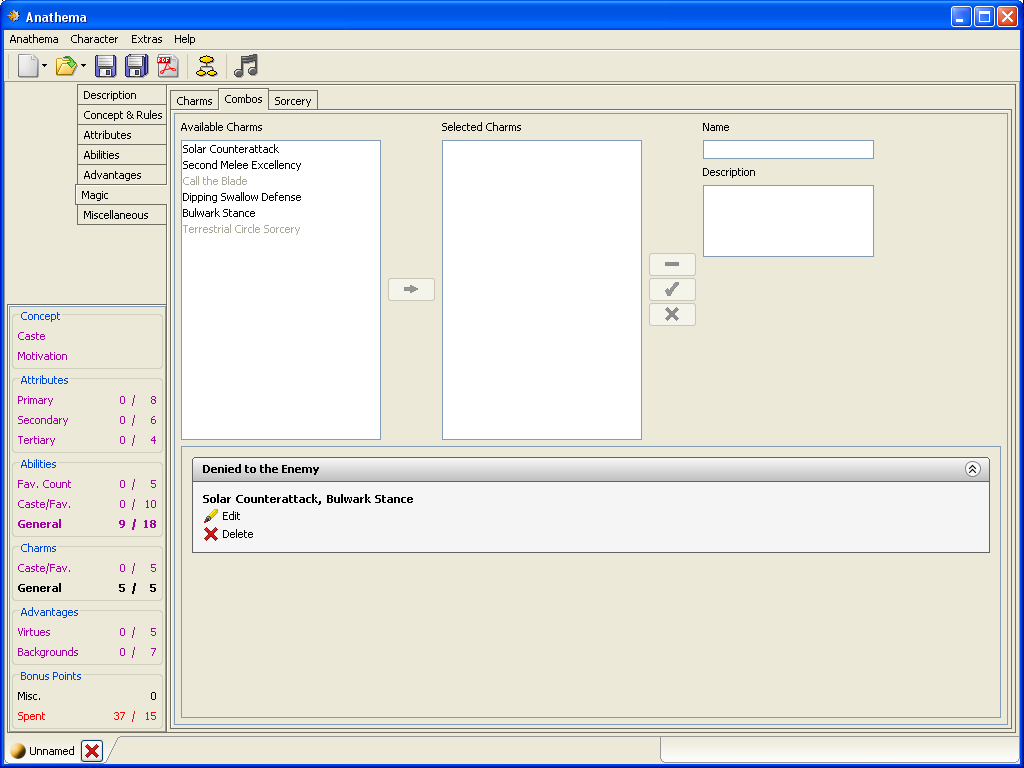
\includegraphics[width=1.00\textwidth]{images/Combos.png}
	\caption{Combos Screen}
	\label{fig:Combos}
\end{figure}

Once the Combo has been finalized it will show up in the list beneath the creation windows. Clicking the  "`edit"' icon will bring it back up, allowing you to change combos later on. Note that while editing, the "`clear"' button is replaced with an option to "`revert all changes"'.

\subsection{Advantages}
\subsubsection{Backgrounds}
Not every Background from the books is listed, but new ones can easily be added. You can also add text to the backgrounds listed to indicate exactly what they are. 

The program will not allow a single background to be chosen more than once. This limitation can be circumvented by customizing your entries.

\subsection{Miscellaneous}
\subsubsection{Equipment}
You can equip previously created items on a character. The items you made will appear on the left and can be added to the character's inventory (on the right) using the customary green arrow. 

The inventory will show items with all of their stats listed. The checkbox in front of each set of statistics is used to mark the set for printing. Checked stats will appear on the character sheet (space permitting) and will be totaled up.  Unchecked items will not print.

\section{Experience}
Once character creation is finished, the character can be further advanced within the program. To do so, you have to convert it to "`experienced mode"' using the "`Character"' menu.
 
After converting, you'll notice a change in the Overview window - instead of listing details of character creation, it now shows your current XP breakdown - as well as a new Experience tab.

Within, you'll find a table in which to enter the experience awards for your character.  To do so, add an entry by clicking the '+' button and adjust the number. You can also add a comment for later reference.

From now on, your character's stats cannot be lowered below the values you've set during creation, and any adjustments you make will be paid for with experience, their cost being calculated automatically. 

You can use the table to keep track of negative XP to cover for expenses not supported by the program.   

\begin{figure}
	\centering
		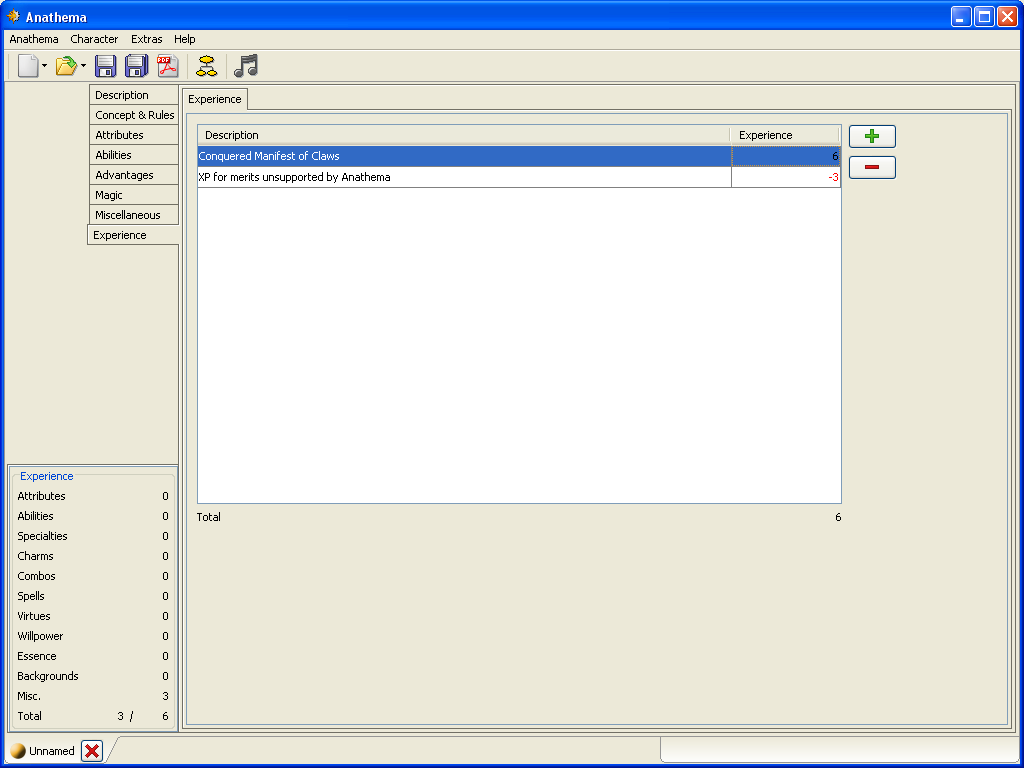
\includegraphics[width=1.00\textwidth]{images/Experience.png}
	\caption{Gaining and spending experience}
	\label{fig:Experience}
\end{figure}

\section{Printing Options}
Characters can be printed in three different ways, choosing from two styles of character sheets and a plain-text "`Character Description"'.